\documentclass[preprint,12pt,aps,pra,showkeys,amsmath,amssymb,superscriptaddress,floatfix]{revtex4-2}
\usepackage[T1]{fontenc}
\usepackage[utf8]{inputenc}
\usepackage{amsmath,amssymb,amsthm,mathtools,mathrsfs}
\usepackage{microtype,booktabs,enumitem}
\usepackage{xcolor,tikz,etoolbox}
\usepackage[skins,breakable]{tcolorbox}
\usepackage{needspace}
% Keep diagram geometry independent of REVTeX preprint body spacing.
\AtBeginEnvironment{tikzpicture}{\linespread{1}\selectfont}
\usetikzlibrary{arrows.meta,positioning,calc,fit,decorations.pathreplacing}
\usepackage{graphicx}
\usepackage{hyperref}

\definecolor{MMBlue}{RGB}{0,82,155}
\definecolor{MMOrange}{RGB}{200,80,0}
\tikzset{
 mmnode/.style={draw=MMBlue,rounded corners=2pt,fill=MMBlue!4,align=left,execute at begin node={\raggedright},text width=5cm,font=\fontsize{10}{12}\selectfont,inner sep=6pt},
 mmimport/.style={mmnode,draw=black!65,fill=black!4},
 mmcandidate/.style={mmnode,draw=MMOrange,dashed,fill=MMOrange!5},
 mmrejected/.style={mmnode,draw=black,densely dotted,fill=black!8},
 mmproof/.style={->,thick,MMBlue},
 mmflow/.style={->,semithick,black!70},
 mmrepair/.style={->,dashed,thick,MMOrange},
 mmcandidatearrow/.style={->,dashed,semithick,MMOrange},
 mmnote/.style={font=\scriptsize,fill=white,inner sep=2pt,align=center}}

\usepackage[section]{placeins}
\setlength{\emergencystretch}{3em}
\setlist{itemsep=3pt,topsep=4pt}
\newtheorem{theorem}{Theorem}[section]
\newtheorem{proposition}[theorem]{Proposition}
\newtheorem{lemma}[theorem]{Lemma}
\newtheorem{corollary}[theorem]{Corollary}
\theoremstyle{definition}
\newtheorem{definition}[theorem]{Definition}
\newtheorem{example}[theorem]{Example}
\theoremstyle{remark}
\newtheorem{remark}[theorem]{Remark}
% Avoid isolated statement headings and single-line paragraph fragments.
\BeforeBeginEnvironment{theorem}{\Needspace{6\baselineskip}}
\BeforeBeginEnvironment{definition}{\Needspace{5\baselineskip}}
\BeforeBeginEnvironment{proposition}{\Needspace{5\baselineskip}}
\BeforeBeginEnvironment{lemma}{\Needspace{5\baselineskip}}
\BeforeBeginEnvironment{corollary}{\Needspace{5\baselineskip}}
\clubpenalty=5000
\widowpenalty=5000
\newcommand{\R}{\mathbb R}\newcommand{\Z}{\mathbb Z}\newcommand{\N}{\mathbb N}
\newcommand{\Pa}{\operatorname{Pa}}\newcommand{\Desc}{\operatorname{Desc}}
\newcommand{\cl}{\operatorname{cl}}\newcommand{\cost}{\operatorname{cost}}
\newcommand{\status}{\operatorname{status}}
% Faculty cards: a visual rail groups the five faculties within one agent.
% The rail has no arrowhead and does not represent a proof dependency.
\newcommand{\mmfacultybadge}[1]{%
 \node[circle,draw=MMBlue,line width=1pt,fill=white,
 minimum size=7mm,inner sep=0pt,font=\sffamily\small\bfseries,text=MMBlue]
 at ([xshift=15pt,yshift=-15pt]frame.north west) {#1};}
\newcommand{\mmfacultyrail}{%
 \draw[MMBlue!80,line width=1pt]
 ([xshift=15pt,yshift=2pt]frame.north west)--
 ([xshift=15pt,yshift=-2pt]frame.south west);}
\newtcolorbox{mmfacultybox}[2]{enhanced,breakable,
 colback=MMBlue!4,colframe=MMBlue!4,boxrule=0pt,arc=3pt,
 left=39pt,right=9pt,top=4pt,bottom=4pt,
 before skip=2pt,after skip=2pt,
 fontupper=\small\linespread{1.1}\selectfont,
 overlay unbroken={\mmfacultyrail\mmfacultybadge{#1}},
 overlay first={\mmfacultyrail\mmfacultybadge{#1}},
 overlay middle={\mmfacultyrail},overlay last={\mmfacultyrail}}
\newcommand{\mmfaculty}[3]{%
 \begin{mmfacultybox}{#1}{#2}
 {\sffamily\bfseries\color{MMBlue}#2}\par\smallskip #3
 \end{mmfacultybox}}
\newcommand{\agent}[9]{%
 \Needspace{8\baselineskip}
 \subsubsection{#1}
 \noindent\textbf{Object.} #2\par
 \noindent\textbf{Role.} #3\par\smallskip
 \mmfaculty{E}{Ego}{#4}
 \mmfaculty{M}{Memory}{#5}
 \mmfaculty{I}{Intellect}{#6}
 \mmfaculty{S}{Sense}{#7}
 \mmfaculty{A}{Action}{#8}
 \smallskip\noindent #9\par}

\usepackage{longtable,array,calc}
\providecommand{\tightlist}{\setlength{\itemsep}{2pt}\setlength{\parskip}{0pt}}
\makeatletter
\def\frontmatter@abstract@produce{\par\addvspace{\frontmatter@preabstractspace}%
\begingroup\prep@absbox\unvbox\absbox\post@absbox\endgroup
\addvspace{\frontmatter@postabstractspace}}
\makeatother
\newcommand{\field}[2]{\par\smallskip\noindent\textbf{#1.} #2\par}
\setlength{\emergencystretch}{5em}
\AtBeginEnvironment{verbatim}{\small\linespread{1.0}\selectfont}


\hypersetup{colorlinks=true,linkcolor=MMBlue,urlcolor=MMBlue,pdfauthor={Dibakar Sigdel}}

\begin{document}

\title{The Gaussian Heat Kernel as an Initial-Value Solution\\[4pt]\large An End-to-End Meta-Math Walkthrough}

\author{Dibakar Sigdel}

\affiliation{Mindverse Computing LLC, Lynnwood, WA 98087, USA}

\date{October 2026}

\begin{abstract}

The Gaussian simultaneously solves the PDE and has total mass one. Its
shrinking tails transfer uniform continuity of the initial data into
uniform convergence. The report presents the target theorem, declared
imports, a dependency graph, five-faculty node contracts, a continuous
proof, a worked example, and a hypothesis-repair audit. It is an
authored mathematical exposition, not a deployed-agent transcript or a
formal proof-assistant certificate.

\end{abstract}\maketitle\linespread{1.12}\selectfont

\noindent\textbf{PDE-04 / Partial Differential Equations / Report v1}

\section{Target and import contract}

\begin{theorem}

For \(\kappa>0\) and bounded uniformly continuous
\(f:\mathbb R^d\to\mathbb R\), define
\(G_t(z)=(4\pi\kappa t)^{-d/2}\exp(-\|z\|^2/(4\kappa t))\) and
\(u(x,t)=\int_{\mathbb R^d}G_t(x-y)f(y)\,dy\) for \(t>0\). Prove this
integral exists, \(u\) is smooth for \(t>0\), \(u_t=\kappa\Delta u\),
\(\|u(\cdot,t)\|_\infty\le\|f\|_\infty\), and \(u(\cdot,t)\to f\)
uniformly as \(t\downarrow0\). This project constructs a solution and
does not assert uniqueness among all unrestricted whole-space solutions.

\end{theorem}

\subsection{Foundations and permitted imports}

Import the Gaussian integral
\(\int_{\mathbb R^d}e^{-\|z\|^2}\,dz=\pi^{d/2}\), Euclidean change of
variables, dominated convergence, and differentiation under an integral
when derivatives have a locally uniform integrable majorant. Polynomials
times Gaussians are integrable; their tails tend to zero by
integrability. Uniform continuity means one \(\delta\) works for all
spatial points.

\clearpage\section{Node interaction workflow}

\begin{center}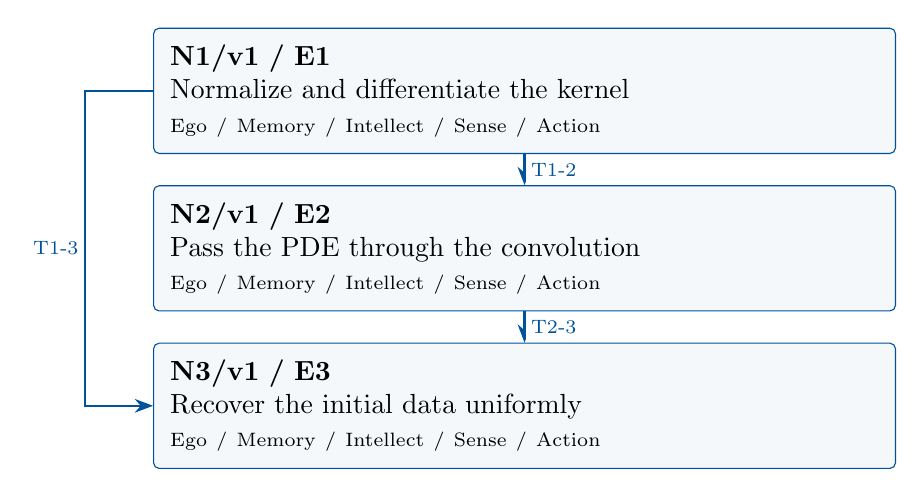
\begin{tikzpicture}[>=Stealth,x=1cm,y=1cm]

\node[mmnode,text width=9cm,minimum height=1.25cm] (N1) at (0,0.0) {\textbf{N1/v1 / E1}\\Normalize and differentiate the kernel\\{\scriptsize Ego / Memory / Intellect / Sense / Action}};

\node[mmnode,text width=9cm,minimum height=1.25cm] (N2) at (0,-2.0) {\textbf{N2/v1 / E2}\\Pass the PDE through the convolution\\{\scriptsize Ego / Memory / Intellect / Sense / Action}};

\node[mmnode,text width=9cm,minimum height=1.25cm] (N3) at (0,-4.0) {\textbf{N3/v1 / E3}\\Recover the initial data uniformly\\{\scriptsize Ego / Memory / Intellect / Sense / Action}};

\draw[mmproof] (N1.south) -- node[mmnote,right] {T1-2} (N2.north);

\draw[mmproof] (N1.west) -- (-5.58,0) -- node[mmnote,left] {T1-3} (-5.58,-4) -- (N3.west);

\draw[mmproof] (N2.south) -- node[mmnote,right] {T2-3} (N3.north);

\end{tikzpicture}\end{center}

Each box is one mathematical agent containing all five faculties. Blue
arrows carry the versioned exports listed below. The layout gives a
reading order; only drawn arrows assert dependencies. Diagnostic repair
is separate from the proof DAG.

\subsection{Versioned evidence-transfer ledger}

\begingroup\small\linespread{1.05}\selectfont

\Needspace{5\baselineskip}\field{T1-2: N1/E1/v1 to N2}{\(G_t>0\), \(\int G_t=1\), and \(\partial_tG_t=\kappa\Delta G_t\).}

\field{Receiving activity}{N2.1}

\field{Compatibility}{E1/v1 and bounded \(f\). Check: Time neighborhoods must stay away from
zero; derivative kernels become singular as \(t\downarrow0\).}

\Needspace{5\baselineskip}\field{T1-3: N1/E1/v1 to N3}{\(G_t>0\), \(\int G_t=1\), and \(\partial_tG_t=\kappa\Delta G_t\).}

\field{Receiving activity}{N3.1}

\field{Compatibility}{E1/v1 mass and bounded uniform continuity of \(f\). Check: The same
\(\delta\) must work for every \(x\); pointwise continuity does not
provide a uniform conclusion.}

\Needspace{5\baselineskip}\field{T2-3: N2/E2/v1 to N3}{\(u\) exists absolutely, is smooth for \(t>0\), satisfies the heat
equation, and obeys the sup-norm bound.}

\field{Receiving activity}{N3.1}

\field{Compatibility}{E1/v1 mass and bounded uniform continuity of \(f\). Check: The same
\(\delta\) must work for every \(x\); pointwise continuity does not
provide a uniform conclusion.}

\endgroup

\clearpage\section{Agent roles and five-faculty activities}\begingroup\small\linespread{1.05}\selectfont\setlist{itemsep=1pt,topsep=2pt}

\subsection{N1/v1: Normalize and differentiate the kernel}

\field{Object and role}{Compute the mass by scaling and compare the time derivative with the
spatial Laplacian. \textbf{Local obligation:} \(G_t>0\), \(\int G_t=1\),
and \(\partial_tG_t=\kappa\Delta G_t\).}

\field{Inputs}{\(G_t\) for \(t>0\) and fixed \(\kappa>0\).}

\mmfaculty{E}{Ego}{Publish E1/v1 only after establishing this obligation: \(G_t>0\),
\(\int G_t=1\), and \(\partial_tG_t=\kappa\Delta G_t\).}

\mmfaculty{M}{Memory}{\(G_t\) for \(t>0\) and fixed \(\kappa>0\). Retain the stated
assumptions and import versions.}

\mmfaculty{I}{Intellect}{Compute the mass by scaling and compare the time derivative with the
spatial Laplacian.}

\mmfaculty{S}{Sense}{The coefficient \(4\kappa t\) controls both the mass normalization and
the PDE coefficient.}

\mmfaculty{A}{Action}{Carry out activities N1.1--N1.2 below, retaining each calculation and
construction as evidence.}

\smallskip\noindent\textbf{Numbered mathematical activities}

\begin{enumerate}[label=N1.\arabic*,leftmargin=3.4em]

\item Set \(z=\sqrt{4\kappa t}\,w\). The Gaussian integral gives
\(\int G_t(z)dz=\pi^{-d/2}\int e^{-\|w\|^2}dw=1\). Positivity is
immediate.

\item Differentiation gives
\(\partial_tG_t=G_t(-d/(2t)+\|z\|^2/(4\kappa t^2))\) and
\(\Delta G_t=G_t(-d/(2\kappa t)+\|z\|^2/(4\kappa^2t^2))\). These
formulas prove the PDE identity. Higher derivatives are finite sums of
polynomial factors times a Gaussian with powers of \(t\) in their
coefficients.

\end{enumerate}

\field{Export E1/v1}{\(G_t>0\), \(\int G_t=1\), and \(\partial_tG_t=\kappa\Delta G_t\).}

\field{Acceptance gate}{The coefficient \(4\kappa t\) controls both the mass normalization and
the PDE coefficient.}

\field{Targeted repair}{If the kernel normalization or diffusivity disagrees, recompute both
derivatives and the scaled mass together. Withhold this export and
recheck its descendants after a versioned correction.}

\clearpage

\subsection{N2/v1: Pass the PDE through the convolution}

\field{Object and role}{Bound convolution by kernel mass and justify differentiation on compact
positive-time neighborhoods. \textbf{Local obligation:} \(u\) exists
absolutely, is smooth for \(t>0\), satisfies the heat equation, and
obeys the sup-norm bound.}

\field{Inputs}{E1/v1 and bounded \(f\). Incoming proof exports: E1/v1 at N2.1.}

\mmfaculty{E}{Ego}{Publish E2/v1 only after establishing this obligation: \(u\) exists
absolutely, is smooth for \(t>0\), satisfies the heat equation, and
obeys the sup-norm bound.}

\mmfaculty{M}{Memory}{E1/v1 and bounded \(f\). Incoming proof exports: E1/v1 at N2.1. Retain
the stated assumptions and import versions.}

\mmfaculty{I}{Intellect}{Bound convolution by kernel mass and justify differentiation on compact
positive-time neighborhoods.}

\mmfaculty{S}{Sense}{Time neighborhoods must stay away from zero; derivative kernels become
singular as \(t\downarrow0\).}

\mmfaculty{A}{Action}{Carry out activities N2.1--N2.2 below, retaining each calculation and
construction as evidence.}

\smallskip\noindent\textbf{Numbered mathematical activities}

\begin{enumerate}[label=N2.\arabic*,leftmargin=3.4em]

\item Absolute integrability follows from
\(\int|G_t(x-y)f(y)|dy\le\|f\|_\infty\int G_t=\|f\|_\infty\), which also
proves the sup-norm bound.

\item Fix a compact set of \(x\) values and \(0<a\le t\le b<\infty\). Every
fixed derivative of \(G_t(x-y)\) is bounded there by a constant times a
polynomial in \(\|y\|\) times \(e^{-c\|y\|^2}\), for some \(c>0\):
bounded \(x\) and positive lower and upper time bounds permit absorbing
shifts and powers into a slower Gaussian. Multiplying by bounded \(f\)
gives an integrable majorant. Differentiation under the integral is
therefore valid for every order locally. E1 then gives
\(u_t-\kappa\Delta u=\int(\partial_tG_t-\kappa\Delta G_t)f=0\).

\end{enumerate}

\field{Export E2/v1}{\(u\) exists absolutely, is smooth for \(t>0\), satisfies the heat
equation, and obeys the sup-norm bound.}

\field{Acceptance gate}{Time neighborhoods must stay away from zero; derivative kernels become
singular as \(t\downarrow0\).}

\field{Targeted repair}{If differentiation is justified by pointwise smoothness alone, supply
the positive-time Gaussian majorant before passing the derivative
through the integral. Withhold this export and recheck its descendants
after a versioned correction.}

\clearpage

\subsection{N3/v1: Recover the initial data uniformly}

\field{Object and role}{Split the convolution error into a uniformly small near part and a
vanishing Gaussian tail. \textbf{Local obligation:}
\(\sup_x|u(x,t)-f(x)|\to0\) as \(t\downarrow0\).}

\field{Inputs}{E1/v1 mass and bounded uniform continuity of \(f\). Incoming proof
exports: E1/v1 at N3.1, E2/v1 at N3.1.}

\mmfaculty{E}{Ego}{Publish E3/v1 only after establishing this obligation:
\(\sup_x|u(x,t)-f(x)|\to0\) as \(t\downarrow0\).}

\mmfaculty{M}{Memory}{E1/v1 mass and bounded uniform continuity of \(f\). Incoming proof
exports: E1/v1 at N3.1, E2/v1 at N3.1. Retain the stated assumptions and
import versions.}

\mmfaculty{I}{Intellect}{Split the convolution error into a uniformly small near part and a
vanishing Gaussian tail.}

\mmfaculty{S}{Sense}{The same \(\delta\) must work for every \(x\); pointwise continuity does
not provide a uniform conclusion.}

\mmfaculty{A}{Action}{Carry out activities N3.1--N3.2 below, retaining each calculation and
construction as evidence.}

\smallskip\noindent\textbf{Numbered mathematical activities}

\begin{enumerate}[label=N3.\arabic*,leftmargin=3.4em]

\item Using mass one, write \(u(x,t)-f(x)=\int G_t(z)(f(x-z)-f(x))dz\). Given
\(\varepsilon>0\), choose \(\delta>0\) with
\(|f(x-z)-f(x)|<\varepsilon\) whenever \(\|z\|<\delta\), uniformly in
\(x\). The integral over that region has absolute value at most
\(\varepsilon\).

\item The remaining part has absolute value at most
\(2\|f\|_\infty\int_{\|z\|\ge\delta}G_t(z)dz\). Scaling expresses the
last integral as
\(\pi^{-d/2}\int_{\|w\|\ge\delta/\sqrt{4\kappa t}}e^{-\|w\|^2}dw\),
which tends to zero. The bound is independent of \(x\), proving uniform
convergence. Define \(u(x,0)=f(x)\) to attach the initial data.

\end{enumerate}

\field{Export E3/v1}{\(\sup_x|u(x,t)-f(x)|\to0\) as \(t\downarrow0\).}

\field{Acceptance gate}{The same \(\delta\) must work for every \(x\); pointwise continuity does
not provide a uniform conclusion.}

\field{Targeted repair}{If a point-dependent continuity radius is used in a supremum estimate,
invoke uniform continuity and repeat the split with one global radius.
Withhold this export and recheck its descendants after a versioned
correction.}

\endgroup\clearpage\section{Continuous mathematical proof}\label{sec:proof}

\subsection{N1 --- Normalize and differentiate the
kernel}\label{n1-normalize-and-differentiate-the-kernel}

\begin{enumerate}
\def\labelenumi{\arabic{enumi}.}
\item
  \textbf{N1.1.} Set \(z=\sqrt{4\kappa t}\,w\). The Gaussian integral
  gives \(\int G_t(z)dz=\pi^{-d/2}\int e^{-\|w\|^2}dw=1\). Positivity is
  immediate.
\item
  \textbf{N1.2.} Differentiation gives
  \(\partial_tG_t=G_t(-d/(2t)+\|z\|^2/(4\kappa t^2))\) and
  \(\Delta G_t=G_t(-d/(2\kappa t)+\|z\|^2/(4\kappa^2t^2))\). These
  formulas prove the PDE identity. Higher derivatives are finite sums of
  polynomial factors times a Gaussian with powers of \(t\) in their
  coefficients.
\end{enumerate}

\subsection{N2 --- Pass the PDE through the
convolution}\label{n2-pass-the-pde-through-the-convolution}

\begin{enumerate}
\def\labelenumi{\arabic{enumi}.}
\item
  \textbf{N2.1.} Absolute integrability follows from
  \(\int|G_t(x-y)f(y)|dy\le\|f\|_\infty\int G_t=\|f\|_\infty\), which
  also proves the sup-norm bound.
\item
  \textbf{N2.2.} Fix a compact set of \(x\) values and
  \(0<a\le t\le b<\infty\). Every fixed derivative of \(G_t(x-y)\) is
  bounded there by a constant times a polynomial in \(\|y\|\) times
  \(e^{-c\|y\|^2}\), for some \(c>0\): bounded \(x\) and positive lower
  and upper time bounds permit absorbing shifts and powers into a slower
  Gaussian. Multiplying by bounded \(f\) gives an integrable majorant.
  Differentiation under the integral is therefore valid for every order
  locally. E1 then gives
  \(u_t-\kappa\Delta u=\int(\partial_tG_t-\kappa\Delta G_t)f=0\).
\end{enumerate}

\subsection{N3 --- Recover the initial data
uniformly}\label{n3-recover-the-initial-data-uniformly}

\begin{enumerate}
\def\labelenumi{\arabic{enumi}.}
\item
  \textbf{N3.1.} Using mass one, write
  \(u(x,t)-f(x)=\int G_t(z)(f(x-z)-f(x))dz\). Given \(\varepsilon>0\),
  choose \(\delta>0\) with \(|f(x-z)-f(x)|<\varepsilon\) whenever
  \(\|z\|<\delta\), uniformly in \(x\). The integral over that region
  has absolute value at most \(\varepsilon\).
\item
  \textbf{N3.2.} The remaining part has absolute value at most
  \(2\|f\|_\infty\int_{\|z\|\ge\delta}G_t(z)dz\). Scaling expresses the
  last integral as
  \(\pi^{-d/2}\int_{\|w\|\ge\delta/\sqrt{4\kappa t}}e^{-\|w\|^2}dw\),
  which tends to zero. The bound is independent of \(x\), proving
  uniform convergence. Define \(u(x,0)=f(x)\) to attach the initial
  data.
\end{enumerate}

\hfill$\square$

\section{Worked orchestration}

In one dimension with \(\kappa=1\) and \(f(x)=e^{-x^2}\), completing the
square inside the Gaussian convolution gives
\(u(x,t)=(1+4t)^{-1/2}\exp(-x^2/(1+4t))\). The Gaussian integral
supplies the prefactor. This broadens and decreases in amplitude, tends
to the original Gaussian as \(t\downarrow0\), and direct differentiation
confirms \(u_t=u_{xx}\).

\subsection{Boundary and hypothesis audit}

For discontinuous \(f=1_{(0,\infty)}\) in one dimension, symmetry gives
\(u(0,t)=1/2\) for every \(t>0\), whereas \(f(0)=0\). The uniform
initial-data conclusion is false. The convolution still exists and
solves the PDE at positive time, illustrating which conclusion uses
continuity.

\section{Illustrative failure and repair}

The following is an authored diagnostic scenario. Changed assumptions
define a new contract; they do not retroactively prove the original
statement.

\subsection{Rejected argument, diagnosis, and correction}
\textbf{Rejected N3 claim:} mass one alone implies uniform recovery of
every bounded \(f\). \textbf{Sense witness:} the step function at the
origin. \textbf{Diagnosis:} Intellect omitted the near-field continuity
estimate. \textbf{Repair:} use bounded uniform continuity as explicitly
assumed and the near/tail decomposition. Recheck only the initial-data
export; the positive-time kernel and PDE calculations remain valid under
boundedness.

\subsection{Publication and reuse}
The corrected export retains its explicit assumptions. A hypothetical
revision receives a new version, and each consuming activity is
rechecked; this scenario is not a recorded runtime event. \textbf{Next
direction:} Prove a uniqueness theorem in a specified bounded solution
class, or extend convergence to \(L^p\) initial data using
approximation.

\par\medskip\begingroup\small\linespread{1.0}\selectfont\noindent\textbf{Provenance.} This authored proof is complete relative to its declared imports. Reuse
each export with its assumptions, proof, and version. The original
Markdown remains available for comparison.
\par\endgroup

\par\smallskip\begingroup\small\linespread{1.0}\selectfont\noindent\textbf{Further reading.} \href{https://math.stanford.edu/~lms/lecs-on-pde.pdf}{Leon Simon,
Lectures on PDE}, for elliptic, weak, and parabolic methods. Classical
calculus and the explicitly stated Hilbert-space imports are used below;
the displayed PDE arguments are developed in full.\par\endgroup

\end{document}
